\documentclass[12pt]{article}

\usepackage[
  paperwidth=1189mm,
  paperheight=841mm,
  margin=22mm
]{geometry}
\usepackage{fontspec}
\usepackage{microtype}
\usepackage{xcolor}
\usepackage{graphicx}
\usepackage{tikz}
\usepackage[most]{tcolorbox}
\usepackage{tabularx}
\usepackage{booktabs}
\usepackage{array}
\usepackage{enumitem}
\usepackage{ragged2e}

\usetikzlibrary{arrows.meta, positioning, calc, fit, backgrounds}

\setmainfont{Helvetica Neue}[
  BoldFont = Helvetica Neue Bold,
  ItalicFont = Helvetica Neue Italic
]
\setsansfont{Helvetica Neue}[
  BoldFont = Helvetica Neue Bold,
  ItalicFont = Helvetica Neue Italic
]

\definecolor{Navy}{HTML}{14324A}
\definecolor{DeepNavy}{HTML}{0B2235}
\definecolor{Teal}{HTML}{0F7B78}
\definecolor{Gold}{HTML}{D79322}
\definecolor{Ink}{HTML}{1F2933}
\definecolor{Slate}{HTML}{536575}
\definecolor{Mist}{HTML}{EEF4F6}
\definecolor{Line}{HTML}{CBD7DE}
\definecolor{SoftTeal}{HTML}{E6F3F2}
\definecolor{SoftGold}{HTML}{FFF4DE}
\definecolor{SoftBlue}{HTML}{E9F1F7}
\definecolor{SoftRed}{HTML}{FFF0EA}

\pagestyle{empty}
\setlength{\parindent}{0pt}
\setlength{\parskip}{3pt}
\renewcommand{\familydefault}{\sfdefault}
\setlist[itemize]{leftmargin=*, topsep=1.5mm, itemsep=1.5mm, parsep=0pt}
\setlist[enumerate]{leftmargin=*, topsep=1.5mm, itemsep=1.4mm, parsep=0pt}

\newcommand{\posterbody}{\fontsize{17.4}{21.6}\selectfont}
\newcommand{\smallbody}{\fontsize{14.4}{17.8}\selectfont}
\newcommand{\tinybody}{\fontsize{12.0}{14.5}\selectfont}
\newcommand{\boxhead}[1]{%
  {\color{Navy}\bfseries\fontsize{25.0}{29.0}\selectfont #1}\par
  \vspace{1.4mm}
  {\color{Teal}\rule{\linewidth}{1.1pt}}\par
  \vspace{2.4mm}
}

\newtcolorbox{sectionbox}{
  enhanced,
  colback=white,
  colframe=Line,
  boxrule=0.85pt,
  arc=3mm,
  left=4.3mm,
  right=4.3mm,
  top=4.0mm,
  bottom=4.0mm,
  before skip=0pt,
  after skip=5mm,
  drop fuzzy shadow=black!8
}

\newtcolorbox{metricbox}[1]{
  enhanced,
  colback=#1,
  colframe=#1!80!black,
  boxrule=0.7pt,
  arc=2.4mm,
  left=3mm,
  right=3mm,
  top=2.7mm,
  bottom=2.7mm,
  before skip=0pt,
  after skip=2.5mm
}

\newcommand{\metric}[4]{%
  \begin{metricbox}{#4}
    {\bfseries\fontsize{26}{29}\selectfont\color{DeepNavy} #1}\par
    {\bfseries\smallbody\color{Ink} #2}\par
    {\tinybody\color{Slate} #3}
  \end{metricbox}
}

\newcommand{\evidenceimage}[2]{%
  \begin{minipage}[t]{\linewidth}
    \centering
    \includegraphics[width=\linewidth,height=47mm,keepaspectratio]{#1}\par
    \vspace{1mm}
    {\tinybody\bfseries\color{Ink} #2}
  \end{minipage}
}

\newcolumntype{Y}{>{\RaggedRight\arraybackslash}X}
\newcolumntype{L}[1]{>{\RaggedRight\arraybackslash}p{#1}}

\begin{document}
\posterbody

\begin{tcolorbox}[
  enhanced,
  colback=Navy,
  colframe=Navy,
  boxrule=0pt,
  arc=0mm,
  left=8mm,
  right=8mm,
  top=7mm,
  bottom=7mm
]
  \begin{minipage}[c]{0.115\textwidth}
    \centering
    \colorbox{white}{
\includegraphics[height=45mm]{images/ganesha.jpg}}
  \end{minipage}
  \hfill
  \begin{minipage}[c]{0.675\textwidth}
    {\color{white}\bfseries\fontsize{46}{52}\selectfont
    Perancangan Arsitektur Sistem Otomasi Inspeksi Kontainer di Pelabuhan}\par
    \vspace{3.5mm}
    {\color{white}\fontsize{23}{28}\selectfont
    Aththariq Lisan Quran Daulah Sentono \,|\, 18222013 \,|\, Program Studi Sistem dan Teknologi Informasi, ITB}\par
    \vspace{1.5mm}
    {\color{white!82}\fontsize{17}{21}\selectfont
    Pembimbing: Ir. I Gusti Bagus Baskara Nugraha, S.T., M.T., Ph.D}
  \end{minipage}
  \hfill
  \begin{minipage}[c]{0.17\textwidth}
    \RaggedLeft
    {\color{Gold}\bfseries\fontsize{25}{30}\selectfont Tugas Akhir}\par
    {\color{white}\fontsize{21}{25}\selectfont Cargovision}\par
    \vspace{2mm}
    {\color{white!75}\fontsize{16}{20}\selectfont 2026}
  \end{minipage}
\end{tcolorbox}

\vspace{5mm}

\begin{minipage}[t]{0.285\textwidth}
  \vspace{0pt}
  \begin{sectionbox}
    \boxhead{Masalah Eksisting}
    Proses inspeksi kontainer di pelabuhan masih memiliki titik pencatatan dan
    bukti yang tersebar. Kondisi ini membuat identitas kontainer, dokumen,
    hasil pemeriksaan, dan bukti visual sulit dibaca sebagai satu riwayat yang
    konsisten.
    \begin{itemize}
      \item Dokumen dan formulir masih muncul dalam bentuk fisik atau input manual.
      \item Hasil pemeriksaan visual belum selalu terhubung dengan identitas kontainer yang sama.
      \item Bukti visual, status inspeksi, dan penanggung jawab belum berada pada satu struktur riwayat.
      \item Integrasi dengan sistem pelabuhan perlu diposisikan sebagai kontrak layanan yang bertahap.
    \end{itemize}
  \end{sectionbox}

  \begin{sectionbox}
    \boxhead{Kebutuhan Utama}
    \smallbody
    \renewcommand{\arraystretch}{1.18}
    \begin{tabularx}{\linewidth}{L{0.17\linewidth}Y}
      \toprule
      \textbf{Kode} & \textbf{Makna kebutuhan arsitektur} \\
      \midrule
      KU-01 & Edge, API, web, dan penyimpanan terhubung dalam satu alur inspeksi. \\
      KU-02 & Nomor kontainer menjadi jangkar OCR, pemindaian, dan konteks manifes. \\
      KU-03 & Hasil inspeksi membentuk riwayat kontainer dengan status, waktu, aktor, dan bukti visual. \\
      KU-04 & Data transaksional dan video langsung dipisahkan sesuai karakter beban. \\
      KU-05 & Akses serta aktivitas penting dapat dikendalikan dan ditelusuri. \\
      \bottomrule
    \end{tabularx}
  \end{sectionbox}

  \begin{sectionbox}
    \boxhead{Ruang Lingkup}
    Fokus tugas akhir adalah rancangan arsitektur sistem, model data, alur
    informasi, dan pembagian tanggung jawab antarkomponen. Poster ini tidak
    mengklaim integrasi penuh operasional pelabuhan, akurasi model deteksi pada
    dataset operasional lengkap, atau hasil uji beban lapangan menyeluruh.
    \vspace{2mm}

    \begin{metricbox}{SoftBlue}
      {\bfseries\color{Navy} Fokus objek: kontainer}\par
      Riwayat inspeksi, hasil OCR, hasil pemindaian, manifes, tinjauan manual,
      dan artefak visual dikaitkan kembali ke entitas kontainer.
    \end{metricbox}
  \end{sectionbox}
\end{minipage}
\hfill
\begin{minipage}[t]{0.410\textwidth}
  \vspace{0pt}
  \begin{sectionbox}
    \boxhead{Rancangan Arsitektur Cargovision}
    \centering
    \resizebox{\linewidth}{!}{%
      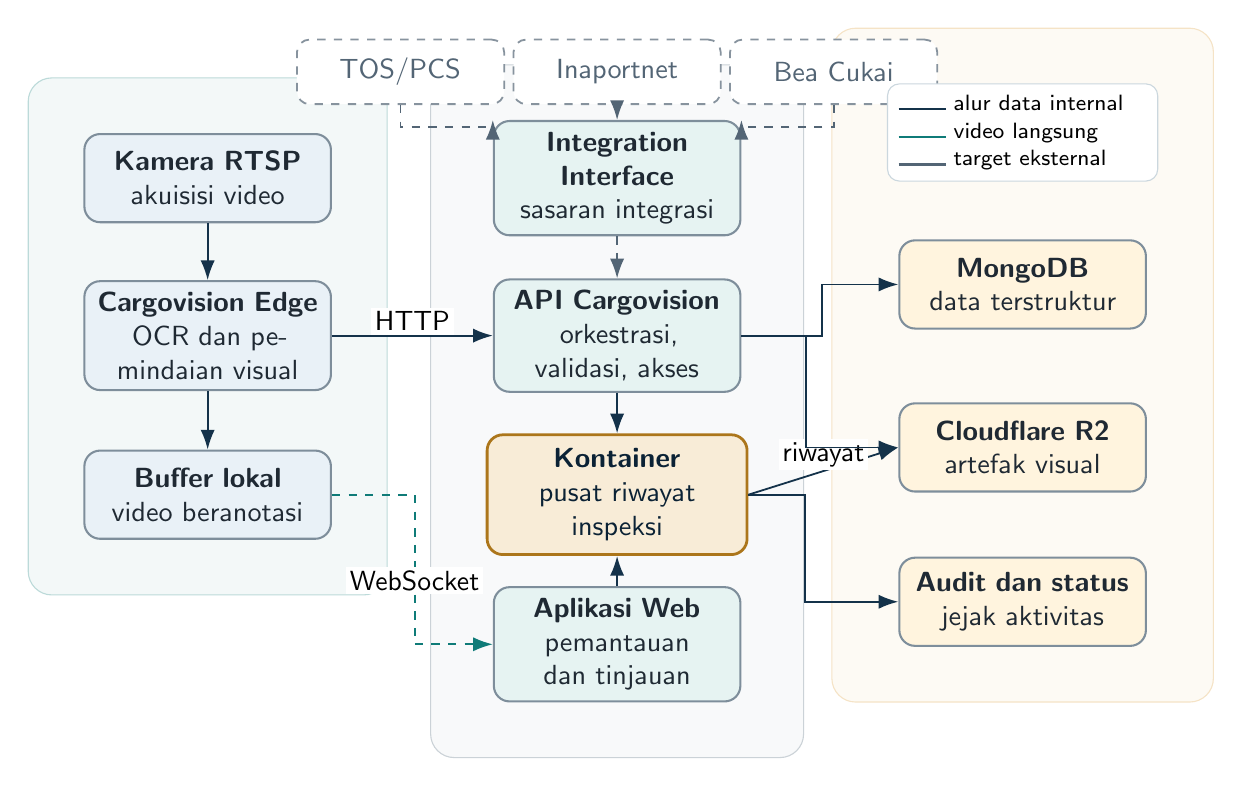
\begin{tikzpicture}[
        x=1cm,
        y=1cm,
        font=\sffamily\fontsize{10.2}{12.2}\selectfont,
        >={Latex[length=2.4mm,width=1.6mm]},
        internal/.style={-{Latex[length=2.5mm,width=1.8mm]}, line width=0.65pt, draw=Navy},
        live/.style={-{Latex[length=2.5mm,width=1.8mm]}, line width=0.65pt, draw=Teal, dashed},
        target/.style={-{Latex[length=2.5mm,width=1.8mm]}, line width=0.65pt, draw=Slate, dashed},
        comp/.style={draw=Navy!55, fill=white, rounded corners=2mm, line width=0.75pt, align=center, text=Ink, inner sep=4pt, minimum height=1.12cm, text width=2.85cm},
        edge/.style={comp, fill=SoftBlue},
        app/.style={comp, fill=SoftTeal},
        data/.style={comp, fill=SoftGold},
        external/.style={draw=Slate!70, fill=white, rounded corners=1.6mm, dashed, line width=0.65pt, align=center, text=Slate, inner sep=4pt, minimum height=0.82cm, text width=2.35cm},
        domainbox/.style={draw=Gold!80!black, fill=Gold!18, rounded corners=2mm, line width=1.0pt, align=center, text=DeepNavy, inner sep=5pt, minimum height=1.25cm, text width=2.95cm}
      ]
        \node[edge] (camera) at (0.0,6.20) {\textbf{Kamera RTSP}\\akuisisi video};
        \node[edge] (edge) at (0.0,4.20) {\textbf{Cargovision Edge}\\OCR dan pemindaian visual};
        \node[edge] (buffer) at (0.0,2.18) {\textbf{Buffer lokal}\\video beranotasi};

        \node[external] (tos) at (2.45,7.55) {TOS/PCS};
        \node[external] (ina) at (5.20,7.55) {Inaportnet};
        \node[external] (customs) at (7.95,7.55) {Bea Cukai};
        \node[app] (interface) at (5.20,6.20) {\textbf{Integration Interface}\\sasaran integrasi};
        \node[app] (api) at (5.20,4.20) {\textbf{API Cargovision}\\orkestrasi, validasi, akses};
        \node[domainbox] (container) at (5.20,2.18) {\textbf{Kontainer}\\pusat riwayat inspeksi};
        \node[app] (web) at (5.20,0.28) {\textbf{Aplikasi Web}\\pemantauan dan tinjauan};

        \node[data] (mongo) at (10.35,4.85) {\textbf{MongoDB}\\data terstruktur};
        \node[data] (r2) at (10.35,2.78) {\textbf{Cloudflare R2}\\artefak visual};
        \node[data] (audit) at (10.35,0.82) {\textbf{Audit dan status}\\jejak aktivitas};

        \node[draw=Line, fill=white, rounded corners=1.5mm, align=left, text width=3.15cm, inner sep=4pt, font=\sffamily\fontsize{8.2}{10}\selectfont] (legend) at (10.35,6.78) {
          \textcolor{Navy}{\rule{6mm}{0.8pt}} alur data internal\\
          \textcolor{Teal}{\rule{6mm}{0.8pt}} video langsung\\
          \textcolor{Slate}{\rule{6mm}{0.8pt}} target eksternal
        };

        \draw[internal] (camera) -- (edge);
        \draw[internal] (edge.east) -- node[above, fill=white, inner sep=1.4pt] {HTTP} (api.west);
        \draw[internal] (edge) -- (buffer);
        \draw[live] (buffer.east) -- ++(1.05,0) |- node[pos=0.24, below, fill=white, inner sep=1.3pt] {WebSocket} (web.west);

        \draw[internal] (api) -- (container);
        \draw[internal] (web.north) -- (container.south);
        \draw[internal] (container.east) -- node[above, fill=white, inner sep=1.3pt] {riwayat} (r2.west);
        \draw[internal] (api.east) -- ++(1.02,0) |- (mongo.west);
        \draw[internal] (api.east) -- ++(0.82,0) |- (r2.west);
        \draw[internal] (container.east) -- ++(0.72,0) |- (audit.west);

        \draw[target] (tos.south) -- ++(0,-0.28) -| (interface.north west);
        \draw[target] (ina.south) -- (interface.north);
        \draw[target] (customs.south) -- ++(0,-0.28) -| (interface.north east);
        \draw[target] (interface) -- (api);

        \begin{scope}[on background layer]
          \node[draw=Teal!28, fill=Teal!5, rounded corners=3mm, fit=(camera)(edge)(buffer), inner sep=7mm] {};
          \node[draw=Navy!22, fill=Navy!3, rounded corners=3mm, fit=(interface)(api)(container)(web), inner sep=7mm] {};
          \node[draw=Gold!26, fill=Gold!5, rounded corners=3mm, fit=(mongo)(r2)(audit)(legend), inner sep=7mm] {};
        \end{scope}
      \end{tikzpicture}
    }
  \end{sectionbox}

  \begin{sectionbox}
    \boxhead{Model Data Berpusat pada Kontainer}
    \begin{center}
    \resizebox{0.98\linewidth}{!}{%
      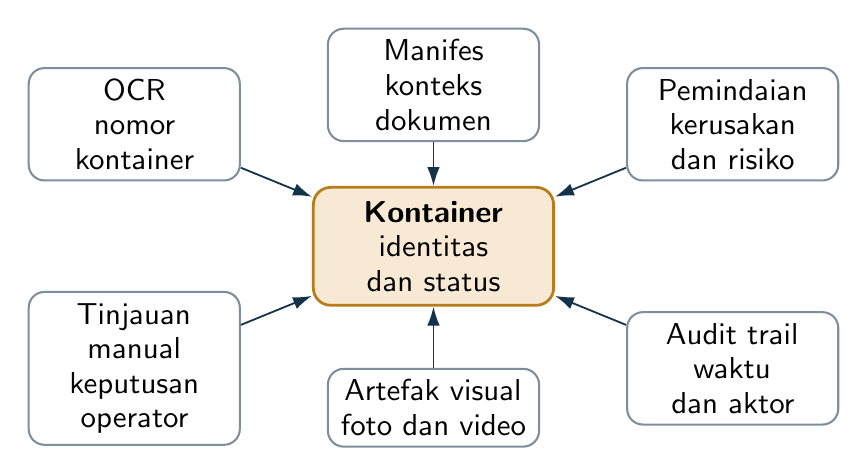
\begin{tikzpicture}[
        font=\sffamily\fontsize{10.5}{12.5}\selectfont,
        rel/.style={-{Latex[length=2.4mm,width=1.6mm]}, line width=0.65pt, draw=Navy},
        entity/.style={draw=Navy!55, fill=white, rounded corners=2mm, line width=0.75pt, align=center, inner sep=4pt, minimum height=0.86cm, text width=2.4cm},
        core/.style={draw=Gold!85!black, fill=Gold!20, rounded corners=2.2mm, line width=1.0pt, align=center, inner sep=5pt, minimum height=1.1cm, text width=2.7cm}
      ]
        \node[core] (container) at (0,0) {\textbf{Kontainer}\\identitas dan status};
        \node[entity] (ocr) at (-3.8,1.55) {OCR\\nomor kontainer};
        \node[entity] (manifest) at (0,2.05) {Manifes\\konteks dokumen};
        \node[entity] (scan) at (3.8,1.55) {Pemindaian\\kerusakan dan risiko};
        \node[entity] (review) at (-3.8,-1.55) {Tinjauan manual\\keputusan operator};
        \node[entity] (visual) at (0,-2.05) {Artefak visual\\foto dan video};
        \node[entity] (audit) at (3.8,-1.55) {Audit trail\\waktu dan aktor};
        \draw[rel] (ocr) -- (container);
        \draw[rel] (manifest) -- (container);
        \draw[rel] (scan) -- (container);
        \draw[rel] (review) -- (container);
        \draw[rel] (visual) -- (container);
        \draw[rel] (audit) -- (container);
      \end{tikzpicture}
    }
    \end{center}
    Entitas kontainer menjadi pusat agregasi. OCR, manifes, hasil pemindaian,
    tinjauan manual, bukti visual, dan audit tidak berdiri sendiri, melainkan
    dibaca sebagai bagian dari riwayat kontainer yang sama.
  \end{sectionbox}

  \begin{sectionbox}
    \boxhead{Alur Inspeksi Ringkas}
    \begin{enumerate}
      \item Kamera mengirim video ke komponen edge untuk OCR dan pemindaian awal.
      \item API memvalidasi hasil, membentuk atau memperbarui entitas kontainer.
      \item MongoDB menyimpan data terstruktur, sedangkan R2 menyimpan artefak visual.
      \item Aplikasi web membaca riwayat kontainer dan menerima video beranotasi melalui WebSocket.
    \end{enumerate}
  \end{sectionbox}
\end{minipage}
\hfill
\begin{minipage}[t]{0.285\textwidth}
  \vspace{0pt}
  \begin{sectionbox}
    \boxhead{Keputusan Arsitektural}
    \begin{itemize}
      \item \textbf{Pemisahan edge dan pusat.} Fungsi sensitif latensi ditempatkan dekat kamera, sedangkan konsolidasi data berada di layanan pusat.
      \item \textbf{Container sebagai jangkar.} Semua hasil inspeksi dikaitkan ke identitas kontainer agar riwayat dapat ditelusuri.
      \item \textbf{MongoDB dan R2 dipisah.} Data terstruktur dan artefak visual memiliki pola penyimpanan dan beban berbeda.
      \item \textbf{HTTP dan WebSocket dipisah.} Data transaksi dikirim lewat API, sedangkan video langsung tidak membebani jalur transaksi.
      \item \textbf{Integrasi eksternal bertahap.} Interface disiapkan untuk TOS/PCS, Inaportnet, dan Bea Cukai tanpa mengklaim integrasi penuh.
    \end{itemize}
  \end{sectionbox}

  \begin{sectionbox}
    \boxhead{Evaluasi Rancangan}
    \metric{96}{kontainer/jam}{kondisi terbaik, satu jalur, 30 detik/kontainer, utilisasi 0,80}{SoftTeal}
    \metric{42}{kontainer/jam}{kondisi nominal, satu jalur, 60 detik/kontainer, utilisasi 0,70}{SoftBlue}
    \metric{15}{kontainer/jam}{kondisi terburuk, satu jalur, 120 detik/kontainer, utilisasi 0,50}{SoftRed}
    \metric{168}{kontainer/jam}{skalasi empat jalur, 60 detik/kontainer, utilisasi 0,70}{SoftGold}
    \vspace{1mm}
    \smallbody
    Estimasi dihitung dari \texttt{K = (3600 / ts) x n x u}.
    Angka ini berfungsi sebagai bukti rancangan dan batas skenario, bukan klaim
    uji beban operasional final.
  \end{sectionbox}

  \begin{sectionbox}
    \boxhead{Hasil Utama}
    \begin{itemize}
      \item Blueprint arsitektur internal yang menghubungkan edge, API, web, MongoDB, dan R2.
      \item Model data yang menempatkan kontainer sebagai pusat riwayat inspeksi.
      \item Alur informasi yang memisahkan data terstruktur dan video langsung.
      \item Pemetaan kebutuhan, rancangan, dan evaluasi kapasitas berbasis skenario.
      \item Bukti realisasi internal mencakup OCR, pemindaian visual, detail riwayat kontainer, dan penyimpanan artefak visual.
    \end{itemize}
  \end{sectionbox}
\end{minipage}

\end{document}
